\section{Results and Analysis}
\label{sec:results}

\paragraph{Classical structure and feasibility.}
Strict feasible retained states exist on 30/32 instances. Cluster repair improves over coordinate greedy on 25/32, with mean score gain 17.019 (paired bootstrap 95\% CI [12.524,21.552]); collaboration rises descriptively from .475 to .664. These findings establish a meaningful classical counterfactual inside the frozen benchmark, but not superiority over mixed-integer programming, CP-SAT, exhaustive full-instance optimization, or a broad ALNS portfolio. Only 27/32 cluster incumbents satisfy composite feasibility even though all 32 record zero disallowed-mode violations, underscoring why verification and fallback cannot be collapsed into a single metric.

\paragraph{Selective conditional evidence.}
Nine of 32 cases (28.13\%) pass the recorded gate. Across all 32 retained-core comparisons, mean optimum mass is .0223 for uniform and .1522 for $p=2$, a ratio of 6.831$\times$ and paired difference .1299 (95\% CI [.0991,.1640]); the first-hit proxy changes from 36.50 to 12.94 draws (paired difference $-23.56$ [${-39.28},{-8.69}$]). The near-optimal coverage difference is +.0443 [${-.0208},.1120$], whose interval crosses zero. \Cref{fig:qvr} maps all observations: low two-solver ambiguity provides little recorded headroom signal, while positive ambiguity and concentration margins identify candidates subject to the remaining gates; neither region establishes economic value.

\begin{figure*}[t]
\centering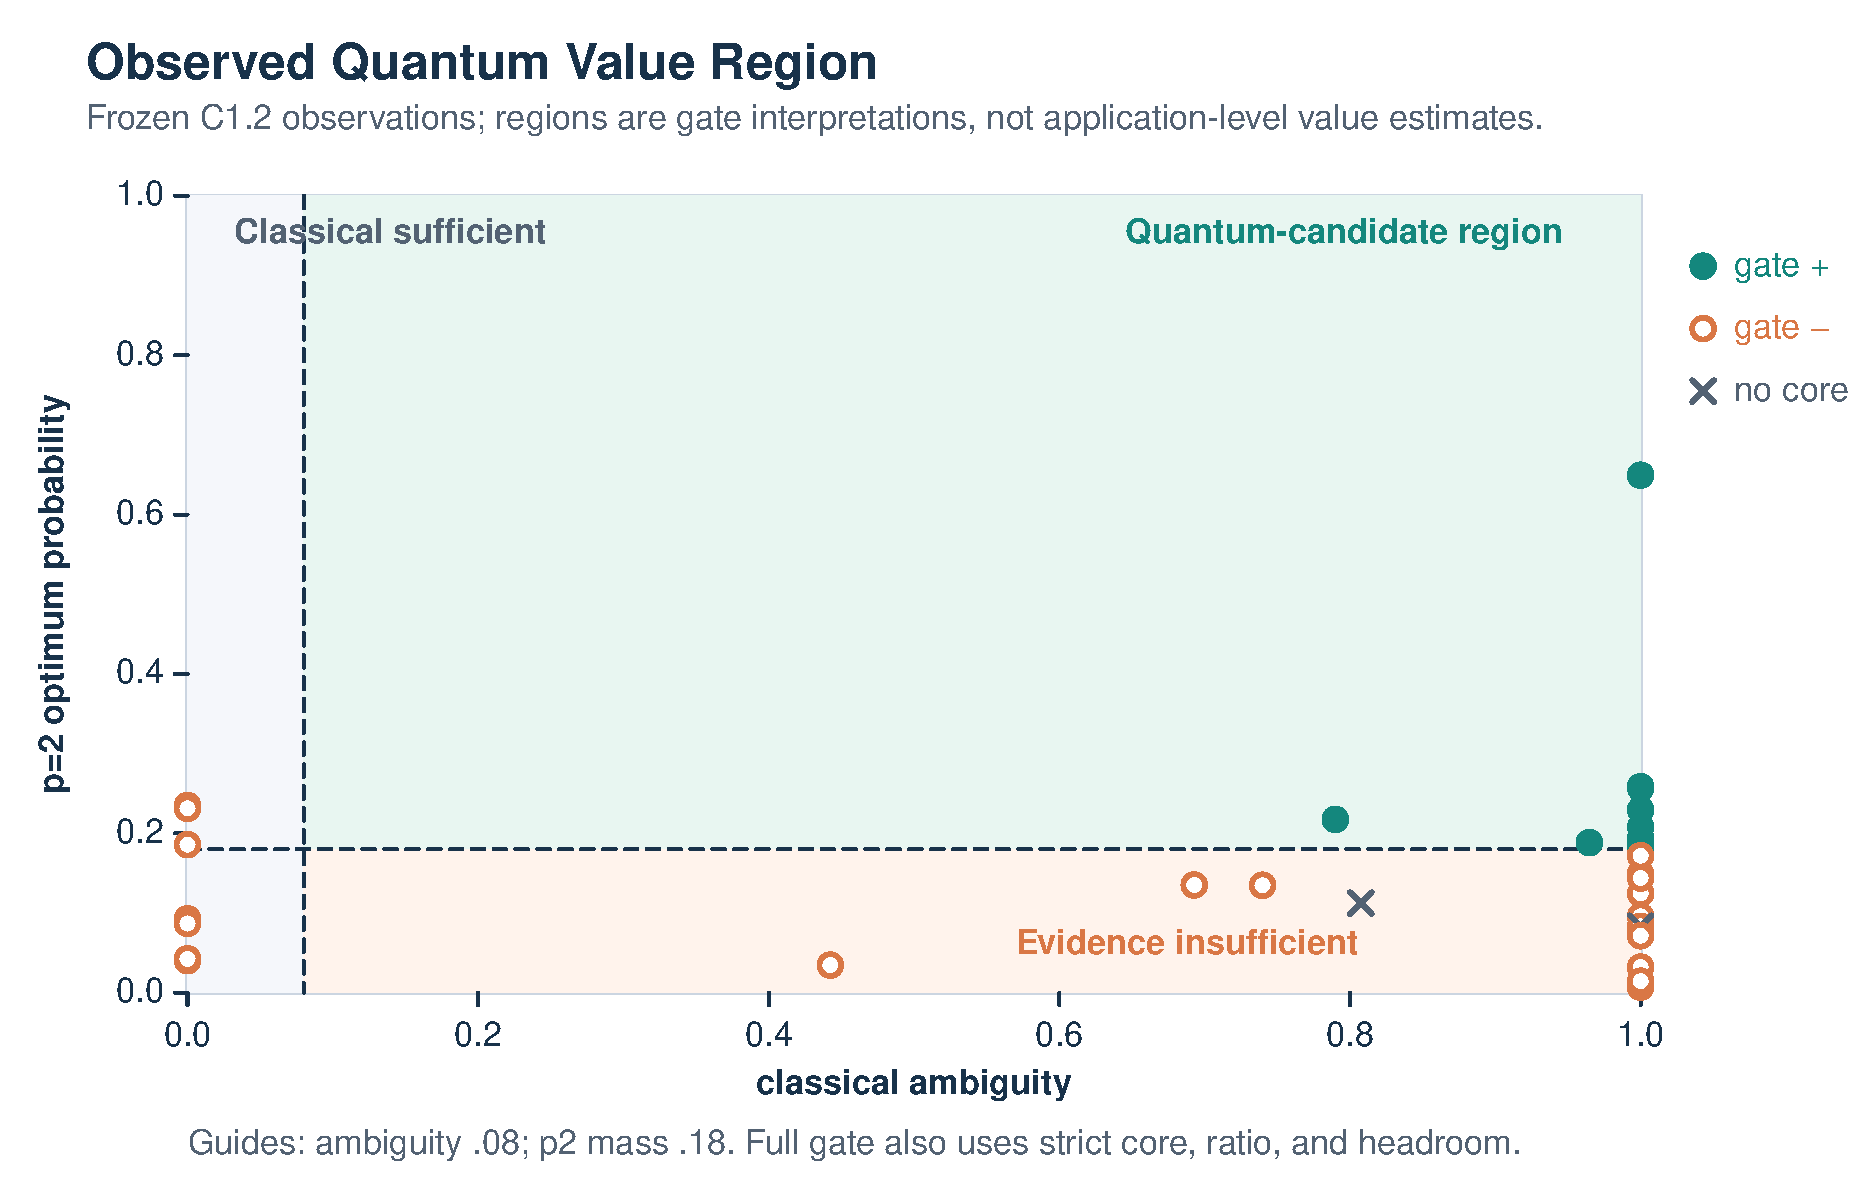
\includegraphics[width=\textwidth]{figs/fig2_quantum_value_region.pdf}
\caption{\textbf{Observed gate diagnostics and the unmeasured economic Quantum Value Region (QVR).} Panel A plots every frozen instance at its ambiguity margin $a-.08$ and concentration margin $p_2^\star-\max(.18,1.4p_U^\star)$. Filled points pass the complete post-simulation gate; open points fail another condition; crosses lack a strict core. Panel B separates the conceptual economic QVR, for which QPU, cost, runtime, risk, review, and stakeholder outcomes were not measured.}\label{fig:qvr}
\end{figure*}

\begin{table}[t]
\caption{Frozen C1.2 benchmark results. Intervals are 95\% paired bootstrap intervals where available; ``-- means no interval was specified.}\label{tab:results}
\footnotesize\setlength{\tabcolsep}{3pt}
\begin{tabularx}{\columnwidth}{@{}Yp{.18\columnwidth}p{.25\columnwidth}Y@{}}
\toprule
\textbf{Metric} & \textbf{Estimate} & \textbf{95\% CI / denominator} & \textbf{Scope} \\
\midrule
Held-out matrix & 32 & -- & Frozen; all cases retained \\
Strict feasible core & 30/32 & -- & Two least-violation fallbacks \\
Cluster repair gain & 17.019 & [12.524, 21.552] & Paired instance bootstrap \\
Uniform optimum mass & 0.0223 & [0.0147, 0.0350] & All retained cores \\
$p=2$ optimum mass & 0.1522 & [0.1161, 0.1940] & Noiseless statevector \\
$p=2$ minus uniform & 0.1299 & [0.0991, 0.1640] & Matched retained state set \\
Evidence-gate positive & 9/32 (28.13\%) & [12.50\%, 43.75\%] & Post-simulation; not prospective \\
Composite-feasible incumbent & 27/32 & -- & Stricter than mode legality \\
Disallowed-mode violations & 0/32 & -- & Not total safety or feasibility \\
\bottomrule
\end{tabularx}
\end{table}


\paragraph{Negative and null evidence.}
The frozen ordered gate failures are two cases without a strict core, seven with low ambiguity, and fourteen with inadequate $p=2$ concentration. The low gate-positive rate is a trust feature only in the limited sense that the recorded gate rejects universal use; because the gate is post-simulation, it does not reduce quantum calls. Mean $p=1$ optimum mass is .2492 and $p=1>p=2$ on 28/32 cases, but the parameter-search budgets differ, so neither deeper-is-better nor shallower-is-better is identified. Uniform feasible sampling is a controlled baseline, not a strong simulated-annealing, tabu, beam-search, or distributional classical portfolio.

\paragraph{What routing evaluation still requires.}
A leakage-free test must freeze a router using pre-execution features and compare Always Classical, Always Quantum, Random, Evidence-Aware, and a hindsight oracle on held-out instances. Coverage $N^{-1}\sum_i\ind[\pi_\tau(z_i)=Q]$, conditional gain, compute/review cost, violations, verification, and fallback should be reported as thresholds vary. The current data cannot support that curve without retrofitting a prospective policy, so Q-OPS reports the test design and limitation rather than inventing points.
